\documentclass[10pt,twocolumn,letterpaper]{article}
\usepackage{cvpr}
\usepackage{times}
\usepackage{graphicx}
\usepackage{amsmath}
\usepackage{amssymb}
\usepackage[pagebackref=true,breaklinks=true,colorlinks,bookmarks=false]{hyperref}

\def\GroupID{XX} % <------- ENTER YOUR COMP6321 group number here

\begin{document}
\title{What {\em is} the Best Classifier?\\
       What {\em is} the Best Regressor?}
\author{Name 1 \and Name 2 \and Name 3\\(if applicable) \and Name 4\\(if applicable)}
\maketitle

\begin{abstract}
   This report investigates two questions.
   First, for a given selection of data sets, can we say what
   is the `best' classifier or the `best' regressor in terms
   of good predictions?
   How much does the answer depend on the particular selection of data sets?
   How much does the answer depend on our computational constraints?
   We investigate these questions using data sets from the UCI repository.
   Second, we compare the interpretability of a decision tree
   classifier to that of a convolutional neural network.
   We compare the decision tree visualization
   to `activation maximization', a technique to gain insight into
   the kinds of inputs that deep neural networks respond to.
\end{abstract}

% DELETE THIS TEXT
The abstract above was drafted for you.
You can submit your project without modifying it, except that you must
add 1--2 sentences to characterize the main idea of your novelty component.
The rest of this template contains a suggested document structure,
but you can change it as you see fit.
Apart from the abstract, You should of course delete the text, formulas, figures, and tables that are currently
included in this template.
The report must be 4 pages of content, plus an additional page for references (if applicable).
Fitting your report into 4 pages may be difficult, as is often the case when writing papers.

%------------------------------------------------------------------------
\section{Introduction}

% DELETE THIS TEXT
Here you should write an introduction to how you approached the project,
as if you were writing a short research paper.
The introduction should be concise but provide an overview of your
goals, your methodology and also provide brief mention of your novelty component.
Even though some of the goals may be mentioned in the abstract,
and some of the methodology is specified in the project guidelines,
you should still try to write this report if it were a paper,
and person reading had not seen the project guidelines.
Describe what you did in your own words, however---copying and pasting is not OK.

% DELETE THIS TEXT
The introduction is not the place for detailed descriptions of data preprocessing,
training, hyperparameter search, testing, or success metrics.
It is OK to mention some specifics if it helps clarify, but the full details
should be explained later on, in the Methodology and Experiments sections.
Likewise you do not need to review your conclusions here---there
is a final section for that.

% DELETE THIS TEXT
The introduction should be 1--1.5 columns in length.



%------------------------------------------------------------------------
\section{Methodology \& Experimental Results}

% DELETE THIS TEXT
Here you'll explain the general aspects of your methodology for determining which
method is best in terms of prediction performance.
In other words, here you can explain aspects that are common to both classification and regression.

\subsection{Classification Experiments}

% DELETE THIS TEXT
Here you'll list the classification data sets (see report guidelines) and explain any methodological
aspects (models evaluated, evaluation metrics used, {\em etc.}) that are specific to classification.
Then you should describe your experimental results,
and reference any relevant figures and/or tables.

\subsection{Regression Experiments}

% DELETE THIS TEXT
Here you'll list the regression data sets (see report guidelines) and explain any methodological
aspects (models evaluated, evaluation metrics used, {\em etc.}) that are specific to regression.
Then you should describe your experimental results,
and reference any relevant figures and/or tables.

\subsection{Interpretability Experiments}

% DELETE THIS TEXT
Here you'll review what you did to process the CIFAR data and train your models.
You should try to give some example of what you saw, in a figure---just enough to get
an idea and to support your conclusions about interpretability.
You'll then state your [hopefully collective] opinion on the interpretability of
these models in particular and on interpretability in general.



%------------------------------------------------------------------------
\section{Conclusions}

% DELETE THIS TEXT
Here you should summarize your thoughts on the questions asked in the abstract.
For which questions can you offer a conclusion or at least a strong opinion?
If a colleague of yours were about to download a dataset like the kind you studied here,
what classifier and training procedure would you recommend he/she use?
What regressor would you recommend, if any?
What model(s) performed the `worst' in your view?
And was the result of your `novelty component'?
Show that you understand what your experimental results imply and do not imply.



\appendix

%-------------------------------------------------------------------------
\section{Detailed experimental results}

% DELETE THIS TEXT
{\em Optional section.} Here you can place supplementary plots and tables if they are needed to
support your conclusions from the main report.
You can include up to 2 extra pages of such material.
They do not count towards your 4-page count.
However, the instructor and TAs should not be obligated to read this
section to understand your conclusions, it should only be used to provide `supplementary' details.
For example, as a full table of your performance results (algorithms $\times$ datasets)
for classification and regression may does not fit within the 4-page limit,
you can put such results here.
If you do not feel including extra figures is necessary, that is OK, just delete this section.


%-------------------------------------------------------------------------
\section{Overview of project code and data}

% DELETE THIS TEXT
{\em Optional section.} This is a guide written by you to help the course staff.
Here you can make a few brief comments to the course staff about where
they should start when looking at your project code, *e.g.* how to run your scripts and what
data files contain the experimental results you used to draw your conclusions.
If your project code already has such information in an obvious place, such as a `README.md`
then this section is not necessary.

%-------------------------------------------------------------------------
\section{Examples of \LaTeX}

% The 'dilde' in Table~\ref{} puts a no-break space prevents "Table" and "1" so that
% the table number does not get split onto a separate line.
% and it is good LaTeX practice to put tildes between 

% DELETE THIS TEXT
This section contains some examples of \LaTeX~to help you get started.
(You should delete this section in the final report.)
This is a reference to Table~\ref{first_table} and Table~\ref{second_table}.
This is a reference to Figure~\ref{first_figure} and Figure~\ref{second_figure}.
This is a citation \cite{breiman2001statistical} and this is
multiple citations \cite{breiman2001statistical,bishop2006pattern}.
This is \textit{italics} and \textbf{bold} text.
This is a formula $\sum_{i=1}^N (y_i - \hat{y}_i(\mathbf{x}))^2$
that is inline with the text (`text style') and this is a
formula that is displayed separately (`display style'):
$$
\sum_{i=1}^N (y_i - \hat{y}_i(\mathbf{x}))^2
$$
These are formulas with an associated equation number
\begin{align}
   \mathbf{x} = \begin{bmatrix}
      x_1, x_2, \ldots, x_N
   \end{bmatrix}^T    \label{xvec}\\
   \boldsymbol{\phi} = \begin{bmatrix}
      \phi_1, \phi_2, \ldots, \phi_M
   \end{bmatrix}^T    \label{phivec}
\end{align}
and we can now refer back to~\eqref{xvec} or to ~\eqref{phivec} like so.



% DELETE THIS TABLE
\begin{table}
   \begin{center}
   \begin{tabular}{|l|c|c|}
   \hline
   Method & Ultra-Clustering & Random Jungles \\
   \hline\hline
   Theirs & Works OK & All your base\\
   Yours & Works better & are belong to us!\\
   Ours & Works best! & I can haz publication?\\
   \hline
   \end{tabular}
   \end{center}
   \caption{This is the caption of a column-width table.\label{first_table}}
\end{table}

% DELETE THIS TABLE
\begin{table*}
   \begin{center}
   \begin{tabular}{|l|c|c|c|}
   \hline
   Method & Good? & Bad? & So-so? \\
   \hline\hline
   Your method & Terrible & Yes, I made sure of it & Star Wars movies \\
   My supervisor's old method (sigh) & I want Tim Horton's & People in hallway... & ...are talking too loudly \\
   My proposed method  & Yes, good! & No, I said good! & What? \\
   \hline
   \end{tabular}
   \end{center}
   \caption{This is the caption of a page-width table.\label{second_table}}
\end{table*}


% DELETE THIS FIGURE
\begin{figure}
   \begin{center}
   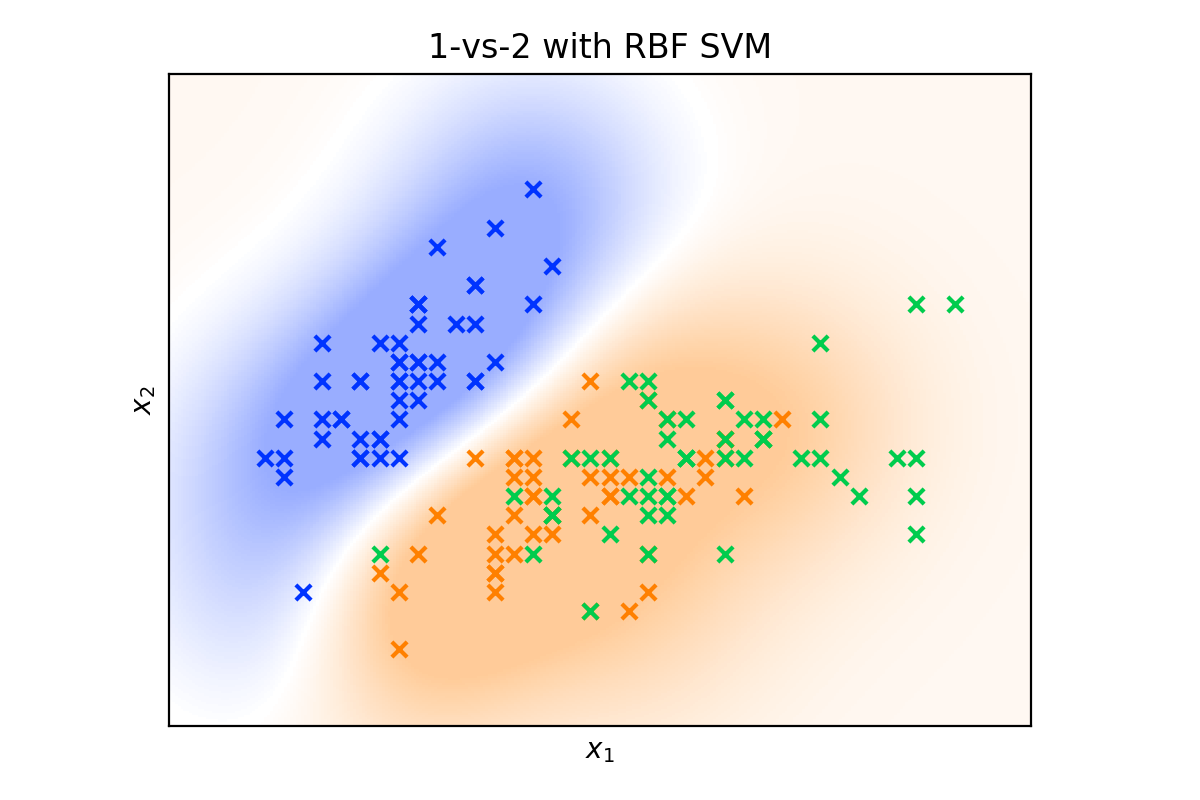
\includegraphics[width=\linewidth]{sample_image.png}
   \end{center}
      \caption{This is the caption of a column-width figure.\label{first_figure}}
\end{figure}
   

% DELETE THIS FIGURE
\begin{figure*}
   \begin{center}
      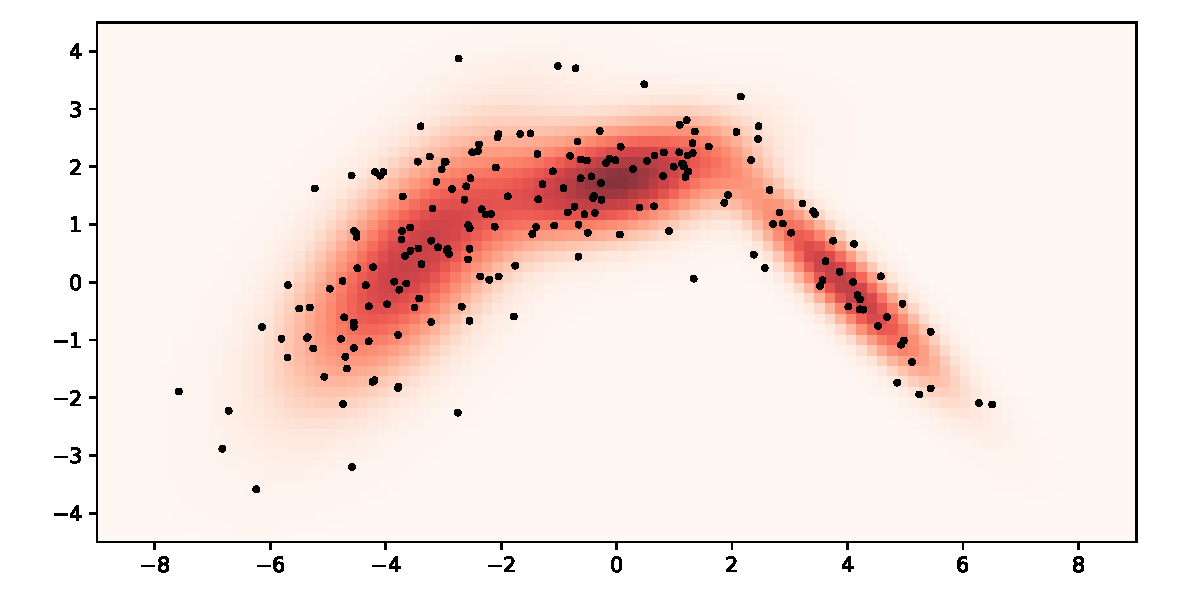
\includegraphics[width=0.4\linewidth]{sample_image.pdf}
      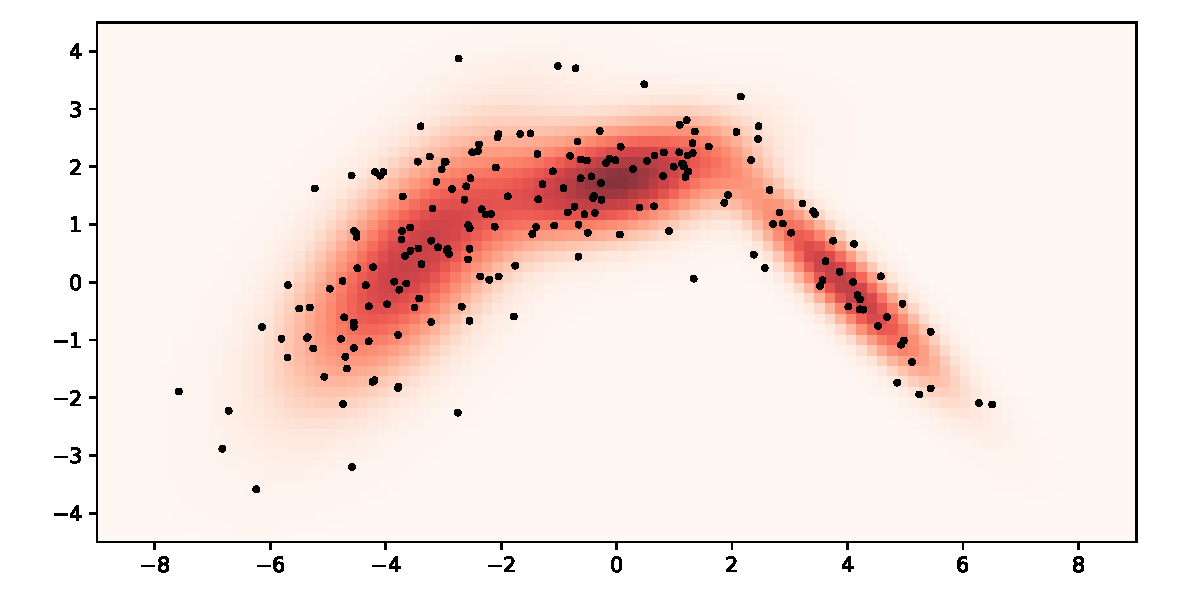
\includegraphics[width=0.4\linewidth]{sample_image.pdf}
   \end{center}
      \caption{This is the caption of a page-width figure.\label{second_figure}}
\end{figure*}





{\small
\bibliographystyle{cvpr_bibstyle}
\bibliography{bibliography}
}

\end{document}
